\section{Pathway Enrichment}\label{sec:pathway_enrichment}
In this section, we start from the gene set obtained in \autoref{sec:geneset_expansion} to find all the disease pathways linked to it, to accomplish that we have used GSEApy, a python package that performs pathway enrichment from many sources. At first we tried with the KEGG and Reactome human datasets with no success since we would have to manually remove all those pathways not related to any disease and there was no way to filter them out, then we found the DisGeNET dataset \cite{disgenet}, which satisfied our needs.
\vspace{3mm}

Passing to the GSEApy \textit{enrichr} method all the nodes in our graph, it performed pathway enrichment on our behalf, then, we filtered the disease pathways by keeping those having a p-value lower than $0.1$, totalling $589$ pathways which will be used during our future network and community analysis.
\vspace{3mm}

An example of disease pathway is in \autoref{fig:example_disease_pathway}, a big number of proteins are do not interact between each other, this is totally normal given the size of our graph and the fact that we centered it around a specific gene and limited it at the second order.
\begin{figure}[H]
    \centering
    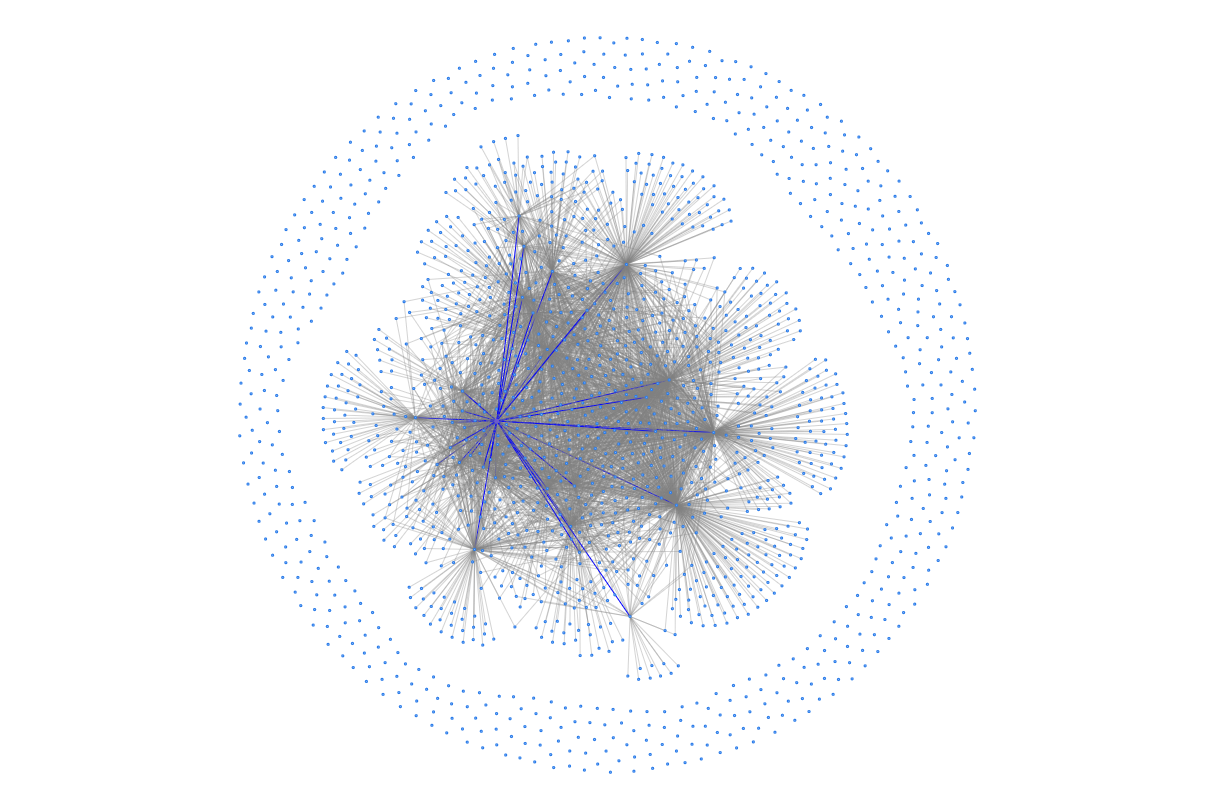
\includegraphics[width=1\linewidth]{images/plots/disease_pathway_graph.png}
    \caption{A disease pathway with the SON gene and its interactions highlighted in blue.}
    \label{fig:example_disease_pathway}
\end{figure}

The GSEApy package, no matter the dataset, always returns a dataframe with following columns (\autoref{fig:disease_pathways} shows such dataframe):
\begin{itemize}
    \item \textbf{Term}, the disease pathway name.
    \item \textbf{Overlap}, the ratio of the disease's genes that are in our graph over the entire number of its gene, the former is more useful than the latter for our analysis.
    \item \textbf{P-value}, how much the result is trustable.
    \item \textbf{Adjusted P-value}, the P-value obtained over all the significant tests.
    \item \textbf{Genes}, a string formed by all the genes of our graph that belong to the pathway, they are comma separated.
\end{itemize}
\begin{figure}[H]
    \centering
    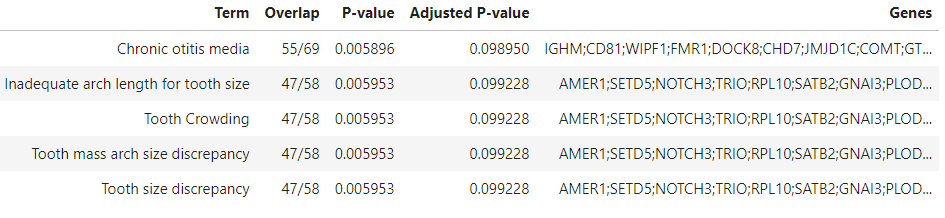
\includegraphics[width=1\linewidth]{images/disease_pathways.png}
    \caption{An example of disease pathways retrieved by using the GSEApy package.}
    \label{fig:disease_pathways}
\end{figure}
Since working with the dataframe genes attribute was not so convenient due to it being a string which we would have to split each time we would have to work with the pathways, we decided to build a dict indexed by the disease's indexes (the first column of the dataframe as seen in \autoref{fig:disease_pathways}) and using the term as the "name" and the splitted genes as a list attribute.